\documentclass[11pt]{article}

\usepackage{sectsty}
\usepackage{graphicx}
\usepackage{subfig}
% Margins
\topmargin=-0.45in
\evensidemargin=0in
\oddsidemargin=0in
\textwidth=6.5in
\textheight=9.0in
\headsep=0.25in

\title{COMP30027: Machine Learning Assignment 1}
\author{ Callum Johnson - 910519 }
\date{\today}

\begin{document}
\maketitle	
\pagebreak

% Optional TOC
% \tableofcontents
% \pagebreak

%--Paper--

\section{Question 1 - Multiclass Evaluation}
Micro-averaging, Macro-averaging and Weighted Averaging was implemented and applied to the Gaussian Naive Bayes Classifier.
For this specific clsasification problem, weighted averaging seems to be the most relevant strategy for comparing classifiers. If we think about the practical applications of an algorithm like this, it is conceivable
that some yoga poses are a lot more rare than others due to being a higher difficulty or just less popular, so it would make sense to prioritise an model that does well on the yoga poses which show up the most.
Note that this logic only holds if the testing data set is a realistic representation of a 'typical' input to our model.

\begin{center}
    \textbf{Multiclass evaluation methods for Gaussian Naive Bayes model}
\end{center}

\begin{figure}[h]
    \centerline{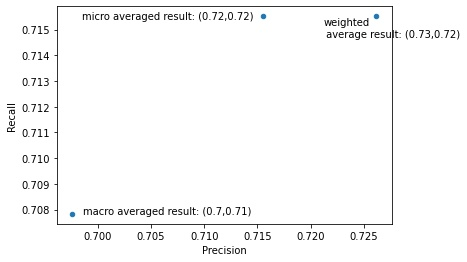
\includegraphics{..\\results\\multiclass_eval_scatter_Gaussian_NB.jpg}}
\end{figure}

\noindent We can see that of the three methods, the weighted averaging strategy produced the highest values for precision and recall. This could be evidence for the model working well for the more common
classes in the test set. If our assumption above about the frequency of different yoga poses is correct, then this would indicate that our model is performing well for classes it is likely to encounter in the real world.
\pagebreak
\section{Question 3 - KDE Classifier}
It was found that without any imputation of missing data, the KDE Classifier
performed slightly more effectively than the Gaussian classifier. The KDE was also ran in comparison to two baseline classifiers, 
one which made random guesses based on the class distribution of the training data, and one which was a standard Zero-R classifier. 
By using the logic detailed in Question 1, the classifiers were compared on the basis of weighted average precision and recall. The raw performance stats were as follows:
\begin{figure}[h]
    \centerline{
\includegraphics[scale = 0.5]{..\\results\\stats_table.png}}
\end{figure}

\noindent The KDE algorithm scored better in both precision and recall over the whole test set, however only marginally. 
Digging deeper, it turns out that this increase was from correctly guessing one instance more than the Gaussian model.
It appeared that there was no major difference in performance between the KDE and Gaussian classifiers across specific classes,
which is shown in the figures below:

\begin{figure}[!ht]
    \centering
    \caption{Precision, Recall comparison for KDE vs Gaussian}
    \subfloat[][]{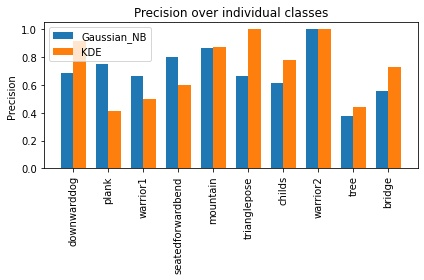
\includegraphics[width=.4\textwidth]{..\\results\\Precision_comparison_Gaussian_NB_KDE.jpg}}\quad
    \subfloat[][]{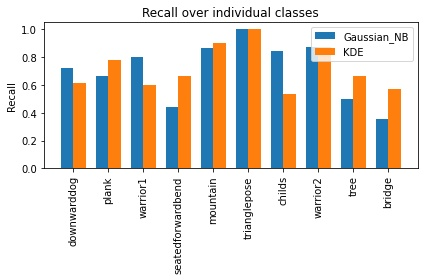
\includegraphics[width=.4\textwidth]{..\\results\\Recall_comparison_Gaussian_NB_KDE.jpg}}\\
    \label{fig:sub1}
\end{figure}

\newpage
\noindent To further demonstrate their similarity, below are the confusion heatmaps for the KDE (left) and Gaussian (right) classifiers:
\begin{figure}[!ht]
    \centering
    \subfloat[][]{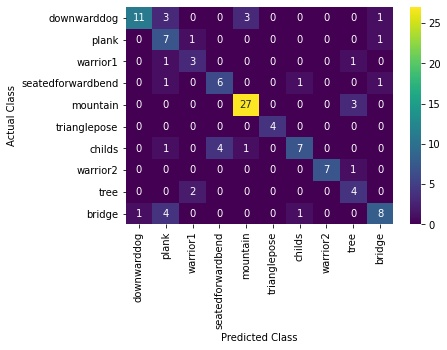
\includegraphics[width=.4\textwidth]{..\\results\\confusion_heatmap_KDE.jpg}}\quad
    \subfloat[][]{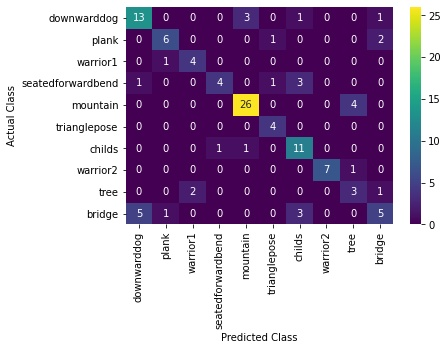
\includegraphics[width=.4\textwidth]{..\\results\\confusion_heatmap_Gaussian_NB.jpg}}\\
    \label{fig:sub1}
\end{figure}

\noindent In terms of actually running the algorithms, the KDE was very slow. In fact the KDE model took around an order of magnitude of
40 - 60 times longer than the Gaussian Naive Bayes. This processing time could be improved by optimising the code with NumPy, however as
it stands this processing time would become a major problem for datasets larger than the provided test set (See table below for time comparisons)

\begin{figure}[h]
    \centerline{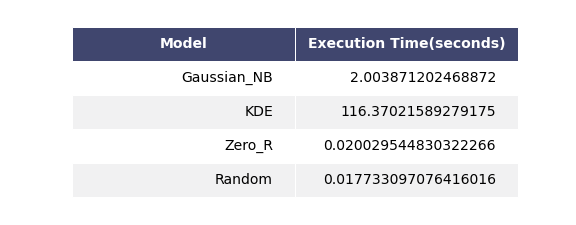
\includegraphics[scale = 0.5]{..\\results\\time_table.png}}
\end{figure}

\end{document}